\documentclass[openany]{book}
% PAQUETES 
\usepackage[utf8]{inputenc}
\usepackage{titling}
\usepackage[spanish]{babel}
\usepackage{amsmath}
\usepackage{graphicx}
\usepackage{hyperref}
\usepackage{float}
\usepackage{amssymb}
%\usepackage{ulem}
\usepackage{ragged2e}
\usepackage{fancyhdr}
\usepackage{hyphenat}
\usepackage{titlesec}
\usepackage{mathtools}
\usepackage{cancel}


\setlength{\textwidth}{130mm}
\setlength{\textheight}{190mm}
\graphicspath{img/}


% RE ESTILIZACION DE COMNADOS
\titleformat 
{\chapter}  %command
[display]  %shape
{\sc\Large}  %format
{Unidad \thechapter}  %label
{0.1pt}  %sep
{
    \rule{\textwidth}{0.5pt}
    \vspace{0.2ex}
    \centering
}  %before-code
\renewcommand{\labelitemi}{$\succ$}
\renewcommand{\chaptermark}[1]{\markboth{\sc #1}{}}
\renewcommand{\sectionmark}[1]{\markright{\sc #1}}

\fancyhf{}
\lhead[\thepage]{\rightmark}
\rhead[\leftmark]{\thepage}
\renewcommand{\headrulewidth}{0.1mm}
\cfoot{{\it Termodinámica de la Atmósfera}}
\renewcommand{\footrulewidth}{0.1mm}

\allowhyphens 

\begin{document}

\begin{titlepage}
	\centering
	{\bfseries\LARGE Universidad Nacional de La Plata \par}
	\vspace{1cm}
	{\scshape\Large Facultad de Ciencias Astronómicas y Geofíscias \par}
	\vspace{3cm}
	{\scshape\Huge Termodinámica de la Atmósfera \par}
	\vspace{3cm}
	{\itshape\Large Resumen teórico \par}
	\vfill
	{\Large Autor: \par}
	{\Large Lorenzo Girotti \par}
	\vfill
	{\Large 2024 \par}
\end{titlepage}

\chapter{Definiciones y escalas. Gases y Ley de Dalton}
\pagestyle{fancy}
\justify
\section{Definiciones básicas}
\begin{itemize}
	\item La {\em termodinámica} estudia el {\em equilibrio de estados} de un {\em sistema} que sufrió algún tipo de {\em transformación de energía}. Específicamente, la termodinámica estudia las transformaciones de calor a trabajo mecánico y viceversa.
	\item Cuando hablamos de {\em sistemas} nos referimos a una muestra determinada de materia. En el caso de la atmósfera, una parcela de aire es un sistema. Un sistema es \emph{abierto} cuando intercambia materia y energía con su entorno; uno \emph{cerrado} es aquel que no intercambia materia. En ese caso, el sistema se compone únicamente de las mismas partículas\footnote{Entiéndase partícula como una masa puntual que puede ser un átomo, una molécula, etc.}. Por practicidad matemática, en la atmósfera consideramos la mayoría de los sistemas como cerrados. Este enfoque se justifica en los siguientes casos: (a) cuando el sistema es suficientemente grande como para ignorar la mezcla con sus alrededores (por ejemplo, una cumulonimbus se puede considerar cerrada, pero una cumulus no); (b) cuando el sistema es parte de un sistema más grande y homogéneo, en cuyo caso la mezcla no modifica significativamente su composición.\par Diremos que un sistema es \emph{aislado} cuando no intercambie ni materia ni energía con su entorno.
	\item Al momento de definir el \emph{estado} de un sistema no podemos adoptar el enfoque de la mecánica clásica, debido a que necesitaríamos conocer la velocidad y la posición de cada una de las partículas que componen nuestro sistema; tarea que en la atmósfera se vuelve absurdamente difícil. Es por ello que en la termodinámica abordamos las propiedades promedio del sistema.\par Si un sistema es un fluido homogéneo compuesto por un solo componente, su estado termodinámico queda definido por su volumen, $V$; su temperatura, $T$; y su presión, $p$. Como $p$, $V$ y $T$ determinan el estado del sistema, deben estar conectadas. Su relación funcional $f(p,V,T)=0$ se llama \emph{ecuación de estado}. De acuerdo con esto, cualquiera de las variables se puede expresar en término de las otras dos. Si tenemos un sistema homogéneo de un solo compuesto, lo podemos describir por completo solo conociendo dos de esas tres variables de estado. Como resultado, obtenemos una forma fácil de estudiar la evolución del sistema mediante un gráfico de $p$ vs $V,$ por ejemplo; en donde la representación de un estado de temperatura constante recibe el nombre de \emph{isoterma}, consecuentemente, podemos definir: \emph{isobara} ($p$ constante), o \emph{isocórica} ($V$ constante).\par En el caso de sistemas que son mezclas de sistemas homogéneos formados por distintos compuestos, además de las variables de estado necesitaremos la concentración de cada uno de ellos. Si el sistema no es homogéneo, deberemos subdividirlo en sistemas que sí lo sean. En ese caso, $p,V$ y $T$ de una subdivisión se vinculan a través de una ecuación de estado.\par Para un sistema cerrado, la composición química y la masa describe al mismo; mientras que su presión, volumen y temperatura describen su estado. Las propiedades que dependen del tamaño del sistema se llaman \emph{extensivas}; mientras que si son independientes del mismo se llaman \emph{intensivas}. Podemos convertir una variable extensiva en intensiva si la dividimos por la masa. A modo de notación, solemos escribir cantidades que dependen de la masa en mayúscula (trabajo $W$, entropía $S$) y las intensivas en minúscula (trabajo específico $w$, calor específico $q$); con excepción de la masa $m$ y la temperatura $T$.
	\item Un \emph{estado de equilibrio} es aquel en donde tanto como las propiedades del sistema como las del entorno permanecen invariables en el tiempo. Puede ser un equilibrio estable, inestable o metaestable. Si es \emph{estable}, pequeños cambios con respecto al equilibrio no remueven al sistema del mismo; si lo hacen, es un equilibrio \emph{inestable}. Decimos que es un equilibrio \emph{metaestable} cuando responde como estable para cierta variación y como inestable para otra.
	\item Una \emph{transformación} lleva al sistema de un estado inicial $i$ a uno final $f$. En un diagrama $(p,V)$ dicha transformación será representada por una curva $I$ que conecta los estados $i$ y $f$. Denotado por $i\xrightarrow{I}f$.\par Una transformación puede ser reversible o irreversible. Decimos que es \emph{reversible} cuando el cambio es paulatino, suave; es decir, le permite tanto al sistema como al entorno ``acomodarse'' y durante cada paso intermedio de la transformación es un estado de equilibrio. Como su nombre lo indica, el cambio se puede revertir a través del mismo camino, invirtiendo los pasos, para devolver al sistema y al entorno al estado inicial. Por otro lado, si el cambio no es paulatino, durante el proceso de transformación los estados intermedios no son estados de equilibrio y por lo tanto, el proceso es \emph{irreversible}.\par Si un sistema va de $i$ a $f$ de forma reversible, puede ir de $f$ a $i$ también reversible si puede realizarse la misma serie de pasos pero en sentido contrario. Si no se pueden invertir los pasos, entonces la transformación se representa mediante otra curva $I'$ en el diagrama $(p,V)$, o sea $f\xrightarrow{I'}i$ y puede ser o no reversible; en otras palabras, el sistema quizás pueda volver a su estado inicial, pero el entorno quizás no.\par Cualquier transformación $ i\rightarrow f\rightarrow i $ se llama \emph{transformación cíclica}. Podemos tener transformaciones cíclicas reversibles o irreversibles.\par Una transformación $i\xrightarrow{I}f$ es \emph{isotérmica} si $I$ es una isoterma; es \emph{isobárica} si $I$ es una isobara; es \emph{isocórica} si $I$ es a volumen constante; y \emph{adiabática} si no se intercambia calor con el entorno.
\end{itemize}

\section{Teoría Cinética del Calor}
Consideremos un sistema a una temperatura $T$ que consiste de $N$ partículas (moléculas). De acuerdo a la teoría cinética del calor, estas moléculas siguen un \emph{movimiento Browniano}\footnote{Movimiento aleatorio en todas las direcciones.}, y por tanto la energía interna de estas partículas no solo difieren entre sí, sino que están en constante cambio con el tiempo. Sin embargo, si calculamos la energía interna \emph{promedio}, vemos que ésta permanece constante con el tiempo. Según la teoría, la energía interna promedio de cada partícula, $\overline{U}$, es proporcional a la temperatura absoluta del sistema, $T$.
\begin{equation}\label{eq:upropt}
	\overline{U}=\mathrm{constante}\times T
\end{equation}
Si asumimos $N\!=\!1$, entonces el punto tiene solo tres \emph{grados de libertad}\footnote{Cantidad de variables independientes requeridas para describir la energía del sistema.}; la velocidad $v$ del punto se puede escribir como
\begin{equation*}
	v^2=v_x^2+v_y^2+v_z^2.
\end{equation*}
Porque solo asumimos una sola partícula, la energía interna total es igual a su energía cinética. Esto es,
\begin{equation*}
	U=\frac{m_p v^2}{2}
\end{equation*}
o
\begin{equation*}
	U_x=\frac{m_p v_x^2}{2},\quad U_y=\frac{m_p v_y^2}{2},\quad U_z=\frac{m_p v_z^2}{2}
\end{equation*}
donde a cada componente le corresponde un grado de libertad.\par De acuerdo al teorema de distribución uniforme de energía, la energía cinética promedio del punto, $ \overline{U}, $ se distribuye equitativamente en los tres grados, i.e. $ \overline{U_x}=\overline{U_y}=\overline{U_z}. $ Entonces, de la ecuación (\ref{eq:upropt}) podemos escribir
\begin{equation*}
	\overline{U_i}=AT,\quad i=x,\,y,\,z
\end{equation*}
donde $A$ es una constante universal (no depende de los grados de libertad, ni del tipo de gas). Esta constante es $k/2$, donde $k$ es la constante de Boltzmann $(k=1.38\times10^{-23}\mathrm{J K}^{-1})$. Entonces, la energía cinética media de un punto con tres grados de libertad es
\begin{equation}
	\overline{U}=\frac{3kT}{2}
\end{equation}
o
\begin{equation*}
	\overline{\frac{m_pv^2}{2}}=\frac{3kT}{2}.
\end{equation*}
El teorema de igual distribución de energía se puede extender a $N$ puntos. En cuyo caso, los grados de libertad serán $3N$ y
\begin{equation*}
	\sum_{i=1}^{N}\overline{\frac{m_pv^2}{2}}=\frac{3NkT}{2}
\end{equation*}
o
\begin{equation*}
	\frac{1}{N}\sum_{i=1}^{N}\overline{\frac{m_pv^2}{2}}=\frac{3kT}{2}
\end{equation*}
o
\begin{equation}
	\left<\frac{\overline{m_pv^2}}{2}\right>=\frac{3}{2}kT
\end{equation}
donde el miembro izquierdo es el promedio de la energía cinética sobre todos los $N$ puntos. Esta ecuación indica que la temperatura absoluta sirve de medida de la energía cinética media de traslación de las moléculas \emph{monoatómicas}; si no lo son, aparecen más grados de libertad que corresponden a otros movimientos como rotaciones sobre el centro de gravedad, oscilaciones alrededor del punto de equilibrio, etc.

\subsection{Gas ideal}
La teoría cinética del calor tiene aplicaciones en la teoría cinética de los \emph{gases ideales}. Un gas ideal cumple que:
\renewcommand{\theenumi}{\alph{enumi}}
\renewcommand{\labelenumi}{({\theenumi})}
\begin{enumerate}
	\item las moléculas se muevan aleatoriamente en todas las direcciones, de manera uniforme; es decir que se mueven la misma cantidad de partículas para cualquier dirección;
	\item mientras se desplazan, las moléculas no ejercen fuerzas; excepto cuando colisionan entre sí o contra las paredes del recipiente que las contiene. Así, el movimiento de cada partícula entre dos choques es lineal y de velocidad uniforme;
	\item los choques entre moléculas son elásticos;
	\item la suma de los volúmenes de las moléculas es despreciable a comparación del volumen de su recipiente.
\end{enumerate}

\section{La primera ley de Gay-Lussac}
A través de experimentos Gay-Lussac pudo demostrar, que a presión constante, el incremento de volumen de un gas ideal, $dV,$ es proporcional al volumen $V_0$ que tiene a una temperatura (medida en escala Celsius) de $\theta=0^{\circ}\mathrm{C}$ y proporcional al incremento de temperatura, $d\theta$:
\begin{equation}\label{eq:d1leygay}
	dV=\alpha V_0d\theta.
\end{equation}
Donde $\alpha$ es el coeficiente de expansión térmico a presión constante y tiene un valor de $1/(273^\circ\mathrm{C})$ para todos los gases.\par
Si integramos (\ref{eq:d1leygay}) obtenemos la relación lineal entre $V$ y $\theta$
\begin{equation*}
	V-V_0=\alpha V_0\theta
\end{equation*}
o
\begin{equation}\label{eq:1leygay}
	V=V_0(1+\alpha\theta)
\end{equation}

\begin{figure}[htbp]
	\centering
	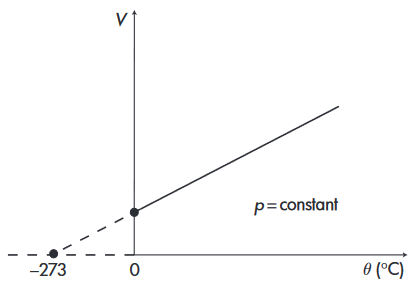
\includegraphics[width=0.5\textwidth]{img/1leygay.png}
	\caption{Representación gráfica de la primera ley de Gay-Lussac}
	\label{fig:1leygay}
\end{figure}

\section{Segunda ley de Gay-Lussac}
Ahora, a volumen constante, Gay-Lussac demostró que el aumento de presión de un gas ideal, $dp$ es proporcional a la presión $p_0$ que tiene el mismo a la temperatura de $0^\circ\mathrm{C}$ y proporcional al aumento de la temperatura $d\theta$:
\begin{equation*}
	dp=\beta p_0d\theta.
\end{equation*}
El coeficiente $\beta$ representa el coeficiente de presión de una expansión térmica a volumen constante y tiene el mismo valor que $\alpha$ para todos los gases.\par
De esta manera, integrando obtenemos
\begin{equation}\label{eq:2leygay}
	p=p_0(1+\beta\theta)
\end{equation}

\section{Temperatura absoluta}
De las ecuaciones (\ref{eq:1leygay}) y (\ref{eq:2leygay}) podemos extrapolar que a $-273^\circ\mathrm{C}$ obtenemos presión y volumen nulos. A ésta temperatura se le llama \emph{cero absoluto}. En base a esto definimos la escala Kelvin para la temperatura absoluta $T=273+\theta$.

\section{Ley de Boyle-Mariotte}
Esta ley nos dice que a temperatura constante, el volumen de un gas es inversamente proporcional a la presión que ejerce.
\begin{equation}\label{eq:boylemariotte}
	pV=p'V',
\end{equation}
donde $p,\,V$ responden a un estado inicial y $p',\,V'$ a uno final.

\section{Ley de gases ideales}
Consideremos un gas ideal en un estado $p,V,T$ el cual es calentado a volumen constante a un estado $p_1,V,T'$. Luego, según la segunda ley de Gay-Lussac (\ref{eq:2leygay})
\begin{equation*}
	p_1=p\frac{T'}{T}.
\end{equation*}
Aumentando su volumen de forma isotérmica, pasamos a un estado $p',V',T'$. Luego según la ley de Boyle-Mariotte (\ref{eq:boylemariotte}),
\begin{equation*}
	p'V'=p_1V.
\end{equation*}
Si combinamos ambos resultados,
\begin{equation*}
	p'V'=p\frac{T'}{T}V
\end{equation*}
o
\begin{equation}\label{eq:leybmgl}
	\frac{pV}{T}=\frac{p'V'}{T'}.
\end{equation}
Llamamos a (\ref{eq:leybmgl}) ``Ley de Boyle-Mariotte-Gay-Lussac'', la cual indica que la relación entre las variables de dos estados se mantiene constante. Lo cual nos invita a escribir
\begin{equation*}
	pV=AT
\end{equation*}
donde $A$ es una constante que depende del tipo y la masa del gas. La dependencia de la masa viene por la \emph{hipótesis de Avogadro}\footnote{El volumen es proporcional a la cantidad de moléculas de un gas.}. Podemos entonces definir $A=mR$ discriminando las dependencias. $R$ se llama \emph{constante específica del gas}. Podemos reescribir entonces, como
\begin{equation}\label{eq:pvmrt}
	pV=mRT.
\end{equation}
Teniendo en cuenta que la masa del gas es $m=Nm_p$ ($N$ partículas de masa $m_p$), podemos pensar a $R=k/m_P$, entonces
\begin{equation}\label{eq:pvnkt}
	pV=NkT.
\end{equation}
Otra forma, es considerando la densidad del gas $\rho=m/V$
\begin{equation}
	p=\rho RT.
\end{equation}
Si definimos \emph{volumen específico} como $a=1/\rho$,
\begin{equation}
	pa=RT
\end{equation}
Si $M$ es la \emph{masa molar} de un gas entonces el número de moles es $n=m/M$. Se deduce la ley como
\begin{equation}
	pV=nMRT,\quad \mathrm{o}\quad pV=nR^*T,\quad \mathrm{o}\quad pa=\frac{R^*}{M}T.
\end{equation}
$R^*=N_Ak$ es la constante universal de los gases y su valor es $R^*=8.3143\,\mathrm{J}/(\mathrm{mol\,K})$.

\section{Ley de Dalton}
Considerando una mezcla de gases que ocupan un volumen $V$ y con $N_1$ y $N_2$ cantidad de moléculas respectivas a los dos gases. Entonces, la presión ejercida sobre las paredes del recipiente será
\begin{equation*}
	p=\frac{(N_1+N_2)}{V}kT\quad \mathrm{o}\quad p=\frac{N_1kT}{V}+\frac{N_2kT}{V}=p_1+p_2.
\end{equation*}
Donde denotamos $p_i$ como la presión parcial que ejerce un gas $i$ a un volumen $V$ y una temperatura $T$.\par
La ley establece que para una mezcla de $r$ componentes (gases ideales), la presión total ejercida por la mezcla es igual a la suma de las presiones parciales ejercidas por cada gas si ocupan todo el volumen a la temperatura de la mezcla.
\begin{equation}
	p=\sum_{i=1}^{r}p_i,
\end{equation}
donde
\begin{equation*}
	p_i=\frac{R^*}{M_i}\frac{m_i}{T}\Rightarrow p=\frac{R^*T}{V}\sum_{i=1}^{r}{\frac{m_i}{M_i}},
\end{equation*}
multiplicando y dividiendo por $m$,
\begin{equation*}
	p=R^*T\frac{m}{V}\frac{\sum_{i=1}^{r}\frac{m_i}{M_i}}{\sum_{i=1}^{r}m_i}=\frac{R^*T}{a}\frac{\sum_{i=1}^{r}\frac{m_i}{M_i}}{\sum_{i=1}^{r}m_i}.
\end{equation*}
Por otro lado, si queremos que la mezcla obedezca la ley de gases ideales,
\begin{equation*}
	p=\frac{RT}{a}=\frac{R^*T}{a\overline{M}}
\end{equation*}
donde $\overline{M}$ es la masa molar media de la mezcla. Igualando, tenemos
\begin{equation}\label{eq:masamolarmezc}
	\overline{M}=\frac{\sum_{i=1}^{r}\frac{m_i}{M_i}}{\sum_{i=1}^{r}m_i}.
\end{equation}
Así, podemos calcular la masa molar de una mezcla de gases que siga la ley de gases ideales, siempre y cuando no haya condensación.\par
Análogamente, podemos encontrar la constante específica de la mezcla,
\begin{equation}
	\overline{R}=\frac{\sum_{i=1}^{r}\frac{m_i}{R_i}}{\sum_{i=1}^{r}m_i}
\end{equation}.

\chapter{Primer Principio de la Termodinámica}
\section{Trabajo}
Como hemos mencionado antes, nuestro enfoque de estudio serán las parcelas de aire. Si una de ellas se encuentra en equilibrio con su entorno, quiere decir que ninguno cambia. Si la presión del entorno cambia, entonces la fuerza asociada al cambio de presión causará perturbaciones en la parcela, desequilibrándola. Para ajustarse a la presión del entorno, la parcela se expandirá $(dV\geq0)$ o se comprimirá $(dV\leq0)$. Al expandirse, la parcela realiza trabajo sobre el entorno; mientras que al comprimirse, es el entorno quien realiza trabajo sobre la parcela. Así definimos
\begin{equation}\label{eq:dW}
	dW=-pdV,
\end{equation}
donde interpretamos que la expansión a la parcela ``le cuesta'' trabajo y por ende el resultado es negativo; mientras que al comprimirse ``gana'' trabajo que fue realizado por el entorno.\par
Integrando de un estado inicial $i$ a uno final $f$
\begin{equation*}
	W=\!\int_{i}^{f}{\!-pdV}
\end{equation*}

\begin{center}
	Si $dV>0$ (el sistema se expande)$\Rightarrow W<0$, el sistema realiza trabajo.\\
	Si $dV<0$ (el sistema se comprime)$\Rightarrow W>0$, el entorno realiza trabajo.
\end{center}
Ahora consideremos una transformación reversible $ i\xrightarrow{I_R}f $ en la cual el sistema se expande y luego se comprime de $f$ a $i$ por la misma transformación, $ f\xrightarrow{I_R}i $, entonces,
\begin{equation*}
	W=\int_{I_R^+}{pdV}+\int_{I_R^-}{pdV}=\int_{I_R^+}{pdV}-\int_{I_R^+}{pdV}=0
\end{equation*}
Sin embargo; si comprimimos a través de otra transformación reversible $ f\xrightarrow{I'_R}i $, entonces
\begin{equation*}
	W=\int_{I_R}{pdV}+\int_{I'_R}{pdV}\neq0
\end{equation*}
Por tanto, $\oint dW=\oint pdV\neq0$ y por lo tanto, $dW$ no es un \emph{diferencial exacto}\footnote{No puede ser función de estado ya que no es independiente a las transformaciones.}, y por tanto lo escribimos $\delta W$ indicando un cambio diferencial de trabajo, pero teniendo en cuenta su naturaleza no conservativa.\par
Si consideramos $dV=dAds$ (donde $dA$ es un diferencial de área y $ds$ uno de distancia), el trabajo queda $ \delta W=pdAds=Fds=Fvdt $ o,
\begin{equation*}
	\frac{\delta W}{dt}=Fv
\end{equation*}
Por la segunda ley de Newton,
\begin{equation*}
	\frac{\delta W}{dt}=m\frac{dv}{dt}v\quad o \quad \frac{\delta W}{dt}=\frac{d}{dt}\left(\frac{1}{2}mv^2\right),
\end{equation*}
entonces tenemos
\begin{equation}\label{eq:trabajoyenergia}
	\frac{\delta W}{dt}=\frac{dK}{dt}
\end{equation}
con $v$ siendo la velocidad de la parcela y $K$ su energía cinética.\par
El resultado nos muestra que una de las formas que tiene un sistema termodinámico de intercambiar energía con su entorno es alrededor es mediante el trabajo realizado.

\section{Definición de energía}
\emph{La primera ley de la termodinámica} enuncia el principio de \emph{conservación de la energía} para sistemas termodinámicos. \textbf{La energía no se crea ni se destruye, se transforma.}\par
Consideremos un sistema cerrado en un entorno adiabático. En este caso, la energía total del sistema $U$ es igual a la suma de la energía potencial y la cinética de sus moléculas. La suma de la energía de todas las moléculas depende del estado en un instante dado, no depende de cómo llegó al mismo.
\begin{equation*}
	\Delta U=U_f-U_i.
\end{equation*}
Si no hay fuerzas externas (el sistema está en equilibrio con su entorno), la energía se conserva ($ \Delta U $).\\
Si hay fuerzas externas, estas realizan trabajo (adiabáticamente)\footnote{Es nuestra hipótesis.} sobre el sistema y según el principio de conservación de energía,
\begin{equation}
	\Delta U=-W^{ad}.
\end{equation}
En este caso particular, el trabajo realizado sólo depende de los estados inicial y final. Entonces, bajo la hipótesis de procesos \emph{adiabáticos}, el trabajo es función de estado.

\section{Equivalencia entre trabajo y calor}
Imaginemos una olla con agua en un estado inicial $T_i$ y uno final $T_f>T_i$. Se puede realizar esta transformación de distintas maneras, la más intuitiva es \emph{calentar} la olla (considerando a $T_f$ lo suficientemente baja como para que no ocurra evaporación). En tal caso, el volumen se mantiene constante y por lo tanto no hay trabajo realizado por fuerzas externas (consideramos también invariante a la presión).\par Otra forma (menos práctica) es tapando la olla de manera que no pueda entrar ni salir agua y agitarla; observaremos que el agua comienza a aumentar su temperatura. Sin embargo, la fricción de las moléculas inhiben el movimiento y por tanto será necesario aplicar trabajo mecánico (agitar) para mantener el movimiento y que siga aumentando la temperatura, hasta alcanzar $T_f$.\par El trabajo realizado por el sistema depende de qué forma elijamos llevar al agua de $i$ a $f$. La energía transmitida al agua en forma de trabajo mecánico por la agitación se transmite mediante una forma no mecánica llamada \emph{calor}.\par \textbf{El calor y el trabajo mecánico, son dos aspectos distintos de la misma cosa: energía.}\par
Para la primera forma,
\begin{equation*}
	\Delta U=Q_{W=0},
\end{equation*}
donde $Q$ es el calor recibido\footnote{Podemos definir al calor necesario para aumentar 1gr de agua en 1°C como \emph{caloría}.}. \par
En la segunda forma,
\begin{equation*}
	\Delta U=-W^{ad}.
\end{equation*}
\par Cuando ambos, trabajo y calor pueden interactuar, obtenemos la expresión general $\Delta U-W=Q$, en forma infinitesimal queda
\begin{equation}\label{eq:1leytermo}
	dU-\delta W=\delta Q,
\end{equation}
de forma equivalente,
\begin{equation}\label{eq:1leytermob}
	dU+pdV=\delta Q\,\xrightarrow{\mathrm{Por\,unidad\,de\,masa\,}}du+pda=\delta q.
\end{equation}
\par Las ecuaciones (\ref{eq:1leytermo}) y (\ref{eq:1leytermob}) representan la forma matemática de la primera ley.

\section{Capacidades térmicas o caloríficas}
Como $dU$ es un diferencial exacto, lo podemos escribir de tres maneras distintas:
\begin{equation}\label{eq:dUforms}
	dU=\frac{\partial U}{\partial T}dT+\frac{\partial U}{\partial V}dV,\quad dU=\frac{\partial U}{\partial T}dT+\frac{\partial U}{\partial p}dp,\, \mathrm{o}\quad dU=\frac{\partial U}{\partial p}dp+\frac{\partial U}{\partial V}dV.
\end{equation}
\par Combinando la primera con la (\ref{eq:1leytermo}) tenemos,
\begin{equation}\label{eq:dQ-TyV}
	\frac{\partial U}{\partial T}dT+\left[p+\frac{\partial U}{\partial V}\right]dV=\delta Q.
\end{equation}
\par Si tenemos en cuenta que $dV(p,T)$ lo podemos obtener a través de la regla de la cadena y combinando la segunda ecuación de (\ref{eq:dUforms}) con la primera ley,
\begin{equation}\label{eq:dQ-pyT}
	\left[\frac{\partial U}{\partial T}+p\frac{\partial V}{\partial T}\right]dT+\left[\frac{\partial U}{\partial p}+p\frac{\partial V}{\partial p}\right]dp=\delta Q.
\end{equation}
\par Por último, si combinamos la primera ley con la tercer ecuación de (\ref{eq:dUforms}) tenemos:
\begin{equation}\label{eq:dQ-pyV}
	\frac{\partial U}{\partial p}dp+\left[\frac{\partial U}{\partial V}-p\right]dV=\delta Q.
\end{equation}
\par Definimos la \emph{capacidad calorífica}, $C$, a la proporción $\delta Q/dT$ y lo notamos como $C_V$ si fue medida a volumen constante; y como $C_p$ si fue a presión constante.\par
De acuerdo a esta definición, si en un sistema a volumen constante no hay cambios del estado físico y químico, entonces el calor absorbido es proporcional a la variación de temperatura.
\begin{equation}\label{eq:dQ-cv}
	\delta Q=C_VdT,\quad\delta Q=c_VmdT,\quad\delta Q=c_{V_m}ndT,
\end{equation}
donde $c_v=C_V/m$ es la capacidad de calor específico y $c_{V_m}=C_V/n$ es la capacidad de calor específico molar.
\par Análogamente, a presión constante:
\begin{equation}\label{eq:dQ-cp}
	\delta Q=C_pdT,\quad\delta Q=c_pmdT,\quad\delta Q=c_{p_m}ndT
\end{equation}
\par Observemos que, si en (\ref{eq:dQ-TyV}) consideramos $dV=0$, tenemos
\begin{equation*}
	C_V=\frac{\delta Q}{dT}=\frac{\partial U}{\partial T},\quad c_V=\frac{\partial u}{\partial T}.
\end{equation*}
\par En (\ref{eq:dQ-pyT}) si reemplazamos $dp=0$
\begin{equation*}
	C_p=\frac{\partial U}{\partial T}+p\frac{\partial V}{\partial T},
\end{equation*}
definiendo una \emph{función de estado}, la \emph{entalpía} como $H=U+pV$, $h=u+pa$, se deduce
\begin{equation*}
	C_p=\frac{\partial H}{\partial T},\quad c_p=\frac{\partial h}{\partial T}.
\end{equation*}
\par Para gases ideales, podemos definir a la entalpía en términos de $(U,V)$ y por tanto, lo podemos expresar como diferencial exacto.
\par Notar que para procesos \emph{isobáricos},
\begin{equation*}
	dH=dU+pdV=\delta Q
\end{equation*}

\subsubsection{Ley de Joule}
Es un experimento que demuestra que la energía interna depende sólo de la temperatura. Imaginemos una cámara aislada de volumen $V$ con un divisor en el medio que separa un gas a presión $p$ del vacío. El gas, se encuentra a una presión $p_i$, ocupando un volumen $V/2$ y a una temperatura $T_i$. Al liberar el gas hacia la otra recámara, el gas pasa a ocupar un volumen $V$ y por tanto disminuye su presión a $p_f$. Entonces tenemos, cambios en la presión y en el volumen pero no se realizó trabajo ni se brindó calor, por lo tanto la energía interna se mantuvo constante, al igual que la temperatura. Por tanto, $U=U(T)$.\vspace{2mm}
\par Teniendo en cuenta esto, las definiciones de $C_V$ y $C_p$ quedan
\begin{equation}\label{eq:cv-dudt}
	C_V=\frac{dU}{dT}\quad c_V=\frac{du}{dT},
\end{equation}
similarmente con la entalpía $H=U+pV=U+nR^*T=H(T)$
\begin{equation}\label{eq:cp-dhdt}
	C_p=\frac{dH}{dT}\quad c_p=\frac{dh}{dT}.
\end{equation}
\par En el rango atmosférico de temperaturas, $C_V$ y $C_p$ son casi constantes, por lo que, integrando (\ref{eq:cv-dudt})
\begin{equation*}
	U=C_VT+\mathrm{constante},
\end{equation*}
como estudiamos variaciones de energía, la constante la vamos a despreciar. Luego, integrando también (\ref{eq:cp-dhdt}) tendremos las siguientes relaciones aproximadas:
\begin{equation*}
	U\approx C_VT\quad H\approx C_pT\quad u\approx c_VT\quad h\approx c_pT
\end{equation*}
\par Combinando (\ref{eq:cv-dudt}) y (\ref{eq:cp-dhdt}) tenemos
\begin{gather}
	\label{eq_cvcpnR}
	C_p-C_V=nR^*,\\
	\label{eq:cvcpR}
	c_p-c_V=R,\\
	\label{eq:cvmcpmR*}
	c_{p_m}-c_{V_m}=R^*.
\end{gather}
\par Recordando que para un gas \emph{monoatómico} que consista en $N$ moléculas, la energía total (interna) es $U=3/2\,NkT$ se deduce,
\begin{gather*}
	C_V=\frac{3}{2}Nk=\frac{3}{2}mR=\frac{3}{2}nMR=\frac{3}{2}nR^*,\\
	c_{V_m}=\frac{3}{2}R^*,\\
	c_V=\frac{3}{2}\frac{n}{m}R^*=\frac{3}{2}R.
\end{gather*}
\par Análogamente,
\begin{gather*}
	C_p=\frac{5}{2}nR^*,\\
	c_{p_m}=\frac{5}{2}R^*,\\
	c_p=\frac{5}{2}R.
\end{gather*}
\par Para gases \emph{diatómicos} los valores cambian a
\begin{gather*}
	C_V=\frac{5}{2}nR^*,\quad c_{V_m}=\frac{5}{2}R^*,\quad c_V=\frac{5}{2}R,\\
	C_p=\frac{7}{2}nR^*,\quad c_{p_m}=\frac{7}{2}R^*,\quad c_p=\frac{7}{2}R.
\end{gather*}
\par Cuando tratamos con cantidades igual a \emph{1 mol}, podemos decir que da igual la definición que usemos para los calores específicos y escribimos
\begin{equation*}
	\frac{C_p}{C_V}=\frac{c_{p_m}}{c_{V_m}}=\frac{c_p}{c_V}=\gamma
\end{equation*}
\\
\par Utilizando las definiciones recién vistas, para gases ideales podemos reescribir la primera ley como
\begin{equation}\label{eq:1leycv}
	C_VdT+pdV=\delta Q\quad c_VdT+pda=\delta q.
\end{equation}
\par Considerando $C_V=C_p-nR^*$ y diferenciando $pV=nR^*T$, reemplazo en la ecuación anterior,
\begin{equation*}
	(C_p-nR^*)dT+(nR^*dT-Vdp)=\delta Q
\end{equation*}
o
\begin{equation}\label{eq:1leycp}
	C_pdT-Vdp=\delta Q
\end{equation}

\begin{table}[!hbt]
	\centering
	\caption{Expresiones de la primera ley.}
	\label{tab:primeraley}
	\begin{tabular}{|l|c|c|}
		\hline Para un gas de masa $m$         & Por unidad de masa                     \\
		\hline $dU-\delta W=\delta Q$          & $ du-\delta w=\delta q $               \\
		$ dU+pdV=\delta Q $                    & $ du+pda=\delta q $                    \\
		$ C_VdT+pdV=\delta Q $\footnotemark[1] & $ c_VdT+pda=\delta q $\footnotemark[1] \\
		$ C_pdT-Vdp=\delta Q $\footnotemark[1] & $ c_pdT-adp=\delta q $\footnotemark[1] \\
		\hline
	\end{tabular}
\end{table}
\footnotetext[1]{Para gases ideales.}

\section{Consecuencias de la primera ley}
Veamos la forma que adquiere la primera ley según los siguientes casos:
\begin{itemize}
	\item Transformaciones isotérmicas: $i\xrightarrow{dT=0}f$.\par Según (\ref{eq:1leycv}), $\delta Q=-\delta W=pdV$, entonces
	      \begin{gather*}
		      Q=\int_{i}^{f}pdV=nR^*T\int_{i}^{f}\frac{dV}{V}\\
		      Q=nR^*T\ln{(V_f/V_i)}
	      \end{gather*}
	\item Transformaciones isocóricas: $i\xrightarrow{dV=0}f$,
	      \begin{gather*}
		      \delta Q=dU=C_VdT\\
		      \Delta U=Q=C_V(T_f-T_i)
	      \end{gather*}
	\item Transformaciones isobáricas: $i\xrightarrow{dp=0}f$
	      \begin{gather*}
		      \delta Q=C_pdT\quad Q=C_p(T_f-T_i)\\
		      \delta W=-pdV\quad W=-p(V_f-Vi)\\
		      \Delta U=C_p\Delta T-p\Delta V
	      \end{gather*}
	\item Transformaciones cíclicas: $i\rightarrow f\rightarrow i$. \par Aquí como $dU$ es diferencial exacto, $\oint dU=0$; luego,
	      \begin{equation*}
		      \oint\delta Q=\oint\delta W
	      \end{equation*}
	\item Transformaciones adiabáticas - Relaciones de Poisson: \par En una transformación adiabática $\delta Q=0$, luego podemos expresar la primera ley como
	      \begin{gather*}
		      dU=\delta W\quad\mathrm{o}\quad C_vdT=-pdV,\\
		      C_pdT=Vdp\quad\mathrm{o}\quad \frac{dT}{T}=\frac{V}{C_p}\frac{dp}{T}.
	      \end{gather*}
	      o utilizando $pV=nR^*T$ y $C_p-C_V=nR^*$
	      \begin{equation*}
		      \frac{dT}{T}=\frac{C_p-C_V}{C_p}\frac{dp}{p}=\left(1-\frac{C_V}{C_p}\right)\frac{dp}{p}
	      \end{equation*}
	      o \begin{equation}
		      \frac{dT}{T}=\left(1-\frac{1}{\gamma}\right)\frac{dp}{p}=\left(\frac{\gamma-1}{\gamma}\right)\frac{dp}{p}
	      \end{equation}
	      Integrando,
	      \begin{gather*}
		      \ln{T}=\left(\frac{\gamma-1}{\gamma}\right)\ln(p)+\ln{(\mathrm{cte})}\\
		      \ln{T}=\ln\left(p^{\frac{\gamma-1}{\gamma}}\right)+\ln{(\mathrm{cte})}\\
		      T=\mathrm{cte}\times p^{\frac{\gamma-1}{\gamma}},
	      \end{gather*}
	      en otras palabras,
	      \begin{equation}\label{eq:poisson1}
		      Tp^{\frac{1-\gamma}{\gamma}}=\mathrm{cte}.
	      \end{equation}
	      Jugando con la ley de gases ideales, llegamos a
	      \begin{gather}
		      TV^{\gamma-1}=\mathrm{cte}, \label{eq:poisson2}\\
		      pV^{\gamma}=\mathrm{cte}.\label{eq:poisson3}
	      \end{gather}
	      Las ecuaciones (\ref{eq:poisson1})-(\ref{eq:poisson3}) expresan las relaciones de Poisson para procesos adiabáticos.
\end{itemize}

\subsubsection{Características del aire seco}
El aire seco se considera diatómico, por lo que $\gamma_d=C_p/C_V=1.4>0$, entonces de la ecuación (\ref{eq:poisson2}) descubrimos que si una parcela se eleva y expande a través de un proceso adiabático, su temperatura debe disminuir para compensar la expansión.
\begin{gather*}
	\gamma_d=1.4\\
	c_{V_d}=718\,\mathrm{J\,kg}^{-1}\mathrm{K}^{-1}=171\,\mathrm{cal\,kg}^{-1}\mathrm{K}^{-1}\\
	c_{p_d}=1005\,\mathrm{J\,kg}^{-1}\mathrm{K}^{-1}=240\,\mathrm{cal\,kg}^{-1}\mathrm{K}^{-1}\\
	R_d=287\,\mathrm{J\,kg}^{-1}\mathrm{K}^{-1}
\end{gather*}
\begin{figure}[hbt!]
	\centering
	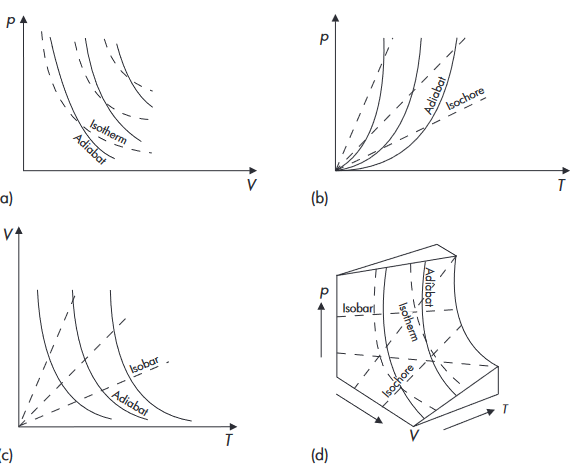
\includegraphics[width=0.7\textwidth]{img/procesos-adiabaticos.png}
	\caption{Relaciones entre variables a través de procesos adiabáticos.}
	\label{fig:rel-adiabaticas}
\end{figure}

\par Debido a que las transformaciones adiabáticas (Fig.\ \ref{fig:rel-adiabaticas}) requieren una aislación perfecta para que no haya intercambios de calor, los procesos adiabáticos son idealizaciones. Sin embargo; para procesos que ocurren rápido, la transferencia de energía es despreciable. Tales procesos son aproximadamente adiabáticos o ``pseudo-adiabáticos''.

\subsection{Gradiente adiabático seco}
De la ecuación (\ref{eq:poisson1}) podemos reescribir,
\begin{gather*}
	T=\mathrm{cte}\,p^{\frac{\gamma-1}{\gamma}}\\
	\ln{T}=\ln{\mathrm{cte}}+\left({\frac{\gamma-1}{\gamma}}\right)\ln{p}\\
	d\ln{T}=\left({\frac{\gamma-1}{\gamma}}\right)d\ln{p}\\
	\frac{dT}{T}=\left({\frac{\gamma-1}{\gamma}}\right)\frac{dp}{p}
\end{gather*}
o
\begin{equation}\label{eq:dpdz-dtdz}
	\frac{1}{T}\frac{dT}{dz}=\left({\frac{\gamma-1}{\gamma}}\right)\frac{1}{p}\frac{dp}{dz}
\end{equation}
\par Por otro lado, para movimientos de aire a gran escala, podemos asumir el \emph{equilibrio hidrostático}:
\begin{equation}
	\label{eq:eq-hidro}
	\frac{dp}{dz}=-\rho g
\end{equation}
donde $\rho$ representa la densidad del entorno. Si consideramos un gas ideal $\rho=p/(RT_E)$, con $T_E$ representando la temperatura del entorno.
\par Entonces, asumiendo procesos adiabáticos, equilibrio hidrostático y un gas ideal, tenemos:
\begin{equation}
	\frac{dT}{dz}=-\left({\frac{\gamma-1}{\gamma}}\right)\frac{g}{R}\frac{T}{T_E}
\end{equation}
\par Recordando que por definición, un ascenso o descenso adiabático es uno en donde no hay intercambio de calor con el entorno. Por tanto, si la parcela se mantiene seca (no hay condensación), podemos definir al \emph{gradiente adiabático seco de temperatura}, $\Gamma_d$, como el perfil vertical de temperatura de la atmósfera tal que la temperatura del entorno sea la misma que la de la parcela $(T=T_E)$, luego
\begin{equation}\label{eq:Gammad}
	\Gamma_d=-\frac{dT}{dz}=\left({\frac{\gamma-1}{\gamma}}\right)\frac{g}{R_d}=\frac{g}{c_{p_d}}=9.8^\circ\mathrm{C\,km}^{-1}
\end{equation}
\par Recordando que $h=u+pa$ y que $h=c_{p_d}T$, podemos reescribir (\ref{eq:Gammad})
\begin{equation}
	\frac{dh}{dz}=-g\quad\mathrm{o}\quad\frac{d}{dz}(h+gz)=0;
\end{equation}
definiendo a $h+gz$ como la \emph{energía estática seca}.
\par Podemos interpretar este resultado de dos maneras: (1) la entalpía de una parcela decrece a medida que asciende adiabáticamente porque realiza trabajo gravitacional; (2) la energía estática se conserva en movimiento adiabático (ascendente o descendente).

\section{Temperatura potencial}
Sea $\theta=ATp^{-\beta}$, con $A$ y $\beta$ constantes. Luego,
\begin{gather*}
	\ln{\theta}=\ln{A}+\ln{T}-\beta\ln{p}\\
	d\ln{\theta}=d\ln{T}-\beta d\ln{p}
\end{gather*}
\par Por otro lado, considerando la primera ley $c_pdT+adp=\delta q$, si dividimos por $T$ y utilizamos la ley de gases ideales, obtenemos
\begin{equation*}
	d\ln{T}+\frac{R}{c_p}d\ln{p}=\frac{\delta q}{c_pT},
\end{equation*}
para $\beta=-R/c_p$,
\begin{equation}\label{eq:thetaq}
	d\ln{\theta}=\frac{\delta q}{c_pT}.
\end{equation}
En procesos adiabáticos $\theta$ se conserva. Podemos definirla de la siguiente manera, de la ecuación (\ref{eq:poisson1}),
\begin{equation*}
	\frac{T}{p^k}=\frac{T_0}{p_0^k},
\end{equation*}
donde $k={\frac{\gamma-1}{\gamma}}=1-\frac{c_V}{c_p}=R/c_p=0.286$ (para aire seco).
\par El estado $(T_0,p_0)$ es un punto de referencia; se elije $p_0=1000\,\mathrm{hPa}$ y $T_0$ queda
\begin{equation*}
	T_0=T\left(\frac{p_0}{p}\right)^k
\end{equation*}
\begin{equation}\label{eq:theta}
	T_0=p_0^k\,Tp^{-k}\xrightarrow[T_0:=\theta]{}\boxed{\theta=p_0^k\,Tp^{-k}}
\end{equation}

\par Llamamos a $\theta$ como la \emph{temperatura potencial}; es la temperatura de una parcela que es llevada de un estado $(T,P)$ al nivel de 1000 hPa a través de un proceso adiabático.
\par En escalas de tiempo en donde una parcela puede considerarse adiabática, los valores constantes de $\theta$ sirven para rastrear los movimientos de ésta. Debido a su dependencia con respecto a $T$ y $p$, su comportamiento será similar al de estos campos; en particular, en la atmósfera: $dp/dz\gg dT/dz$, por lo que las superficies de $\theta$ constantes se asemejan a superficies isobáricas.
\par Extendiendo la idea de la relación entre cambios de temperatura por movimientos verticales de la parcela, la temperatura potencial nos permite interpretarla de la siguiente manera: {\sl durante un ascenso (descenso) adiabático, la temperatura de la parcela deberá disminuir (aumentar) pero en una proporción tal que su temperatura potencial permanezca invariante}.
\par Notar que la ecuación (\ref{eq:thetaq}) indica que para procesos \emph{diabáticos} el cambio de la temperatura potencial es una medida directa del intercambio de calor. Como consecuencia, una parcela bajo condiciones diabáticas atravesará las superficies de $\theta$ constantes en proporción a la cantidad de calor neta intercambiada con su entorno.

\chapter{Segundo Principio de la Termodinámica}
La primera ley, basándose en el principio de conservación de energía, nos dice que: podemos transformar calor en trabajo y trabajo en calor; el trabajo puede realizarse a expensas de la energía interna, y así siguiendo. Esto nos permite describir una gran variedad de fenómenos que ocurren en la realidad. Sin embargo; también nos permite explicar otros que no ocurren. Por ejemplo: un cuerpo pesado que cae al suelo, debido al impacto se calienta (algo que vemos en la realidad); el fenómeno opuesto, un cuerpo en reposo sobre el suelo que comienza a elevarse por sí mismo mientras se enfría (algo imposible), es posible según la primera ley, ya que el trabajo se realiza a expensas de la energía interna del suelo.
\par Requerimos entonces de otra ley que restrinja a la primera y de un sentido formal a los caminos de las transformaciones de energía. Aquí es donde aparece la segunda ley, la cual se encarga de direccionar los procesos termodinámicos y estudia la eficiencia de los mismos. Dado que éstas características controlan el desarrollo de un sistema a partir de un determinado estado, la segunda ley también subyace en la estabilidad del equilibrio termodinámico.
\par Una suerte de simplificación de la segunda ley podría ser el siguiente enunciado: {\sl se puede transformar todo el trabajo en calor; mas no todo el calor en trabajo}.

\section{Procesos naturales y reversibles}
Sabemos que un proceso \emph{reversible} es aquel que le permite al sistema restaurar su estado inicial sin dejar influencia neta sobre el sistema o su entorno. Éste es una idealización: requiere de la ausencia total de fricción y de que los cambios ocurran lo suficientemente lentos para que el sistema no rompa el equilibrio termodinámico.
\par Entendemos entonces, a un proceso \emph{natural} como aquel que se genera libremente, un proceso \emph{espontáneo}. Debido a que el sistema no se encuentra en equilibrio con su entorno, el proceso natural no puede ser revertido completamente (sin dejar influencias sobre el sistema o su entorno). Por lo tanto, un proceso natural es \emph{irreversible}.
\par La irreversibilidad podría darse en cualquier proceso que conduzca al sistema fuera del equilibrio termodinámico. Realizar trabajo a través de una pequeña diferencia de presión lleva al sistema fuera del \emph{equilibrio mecánico}; transferir calor a través de una pequeña diferencia de temperatura conduce a salir del \emph{equilibrio térmico}. Otro cambio irreversible se da cuando ocurren cambios de fase, los cuales se manifiestan ante la presencia de una diferencia de potenciales químicos, rompiendo el \emph{equilibrio químico}.
\par Si alguno de estos tres equilibrios no se cumple, diremos que el sistema no está en equilibrio termodinámico.

\section{Ciclo de Carnot}
El ciclo de Carnot es una idea de motor térmico, que consiste de dos fuentes de calor a distintas temperaturas y un recipiente aislado cuando no interactúa con las fuentes, de mayor eficiencia posible. Es una transformación cíclica que consiste de cuatro pasos (Fig. \ref{fig:ciclo-carnot}).
\renewcommand{\theenumi}{\arabic{enumi}}
\renewcommand{\labelenumi}{\theenumi.}
\begin{enumerate}
	\item Una expansión isotérmica reversible $(1\rightarrow2)$, $T=T_1=\mathrm{cte}$.
	\item Una expansión adiabática reversible $(2\rightarrow3)$, $\theta=\theta_1=\mathrm{cte}$.
	\item Una compresión isotérmica reversible $(3\rightarrow4)$, $T_2<T_1$.
	\item Una compresión adiabática reversible $(1\rightarrow1)$, $\theta_2<\theta_1$.
\end{enumerate}

\begin{figure}[hbt!]
	\centering
	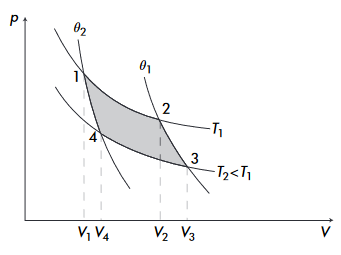
\includegraphics[width=0.5\textwidth]{img/ciclo-carnot.png}
	\caption{Ciclo de Carnot.}
	\label{fig:ciclo-carnot}
\end{figure}

\par Calculemos el trabajo realizado y el calor absorbido cuando un gas ideal realiza este ciclo. Tengamos en cuenta que al ser cíclico, $dU=0$.

\begin{enumerate}
	\item Como es isotérmico, $\Delta T=0$, $Q_{12}=-W_{12}$ por la primera ley y
	      \begin{equation*}
		      W_{12}=-\displaystyle\int_{V_1}^{V_2}pdV=-nR^*T_1\displaystyle\int_{V_1}^{V_2}\frac{dV}{V}=-nR^*T_1\ln{\frac{V_2}{V_1}}.
	      \end{equation*}
	      \par Como $V_2>V_1\Rightarrow W_{12}<0 y Q_{12}>0$ indicando que el gas realizo trabajo de expansión y absorbió calor de la fuente a temperatura $T_1$.
	      \par Por otro lado, $\Delta U_{12}=C_V\Delta T=0$.
	\item Proceso adiabático implica $Q_{23}=0$, entonces $\Delta U_{23}=C_V(T_2-T_1)<0$ y por la primera ley $W_{23}=\Delta U<0$.
	\item Nuevamente, $\Delta T=0\Rightarrow-W_{34}=Q_{34}$
	      \begin{equation*}
		      W_{34}=-nR^*T_2\ln{\frac{V_4}{V_3}}\quad \Delta U=0
	      \end{equation*}
	      \par Como $V_4<V_3$ tenemos $W_{34}>0\Rightarrow Q_{34}<0$ indicando que al contraerse, el entorno ejerce trabajo sobre el gas y éste entrega calor a la fuente $T_2$ para no aumentar su temperatura.
	\item $Q_{41}=0,\quad\Delta U_{41}=C_V(T_1-T_2)>0$, entonces $W_{41}=\Delta U_{41}>0$.
\end{enumerate}
\par Si sumamos todos los trabajos para calcular el trabajo total, tenemos
\begin{equation*}
	W=W_{12}+\cancel{W_{23}}+W_{34}+\cancel{W_{41}}=-nR^*T_1\ln{\frac{V_2}{V_1}}-nR^*T_2\ln{\frac{V_4}{V_3}}
\end{equation*}
\par Como 2. y 4. son adiabáticas, podemos relacionar
\begin{gather*}
	T_1V_2^{\gamma-1}=T_2V_3^{\gamma-1},\\
	T_1V_1^{\gamma-1}=T_2V_4^{\gamma-1}.\\
\end{gather*}
\par Dividiendo ambas ecuaciones,
\begin{equation*}
	\left(\frac{V_2}{V_1}\right)^{\gamma-1}=\left(\frac{V_3}{V_4}\right)^{\gamma-1}\Rightarrow\frac{V_2}{V_1}=\frac{V_3}{V_4}.
\end{equation*}
\par Luego, el trabajo total se puede escribir
\begin{equation*}
	W=-nR^*\ln{\frac{V_2}{V_1}}(T_1-T_2)
\end{equation*}
\par El calor absorbido por el sistema será, debido a que $\Delta U=0$ por ser una transformación cíclica, igual a $-W$, esto es
\begin{equation*}
	Q=nR^*\ln{\frac{V_2}{V_1}}(T_1-T_2)
\end{equation*}

\subsubsection{Rendimiento}
Si consideramos $Q_1=Q_{12}$ al calor brindado por la fuente $T_1$ al sistema y $Q_2=Q_{34}$ al calor que el sistema le entrega a $T_2$, podemos definir la \emph{eficiencia} o el \emph{rendimiento} del ciclo de Carnot, como
\begin{equation}\label{eq:rendimientoQ}
	\eta=\frac{Q_1+Q_2}{Q_1}=1+\frac{Q_2}{Q_1}\quad (Q_1>0,\,Q_2<0)
\end{equation}

Si consideramos la expresión que derivamos para $Q$, tenemos
\begin{equation}\label{eq:rendimientoT}
	\eta=1-\frac{T_2}{T_1}.
\end{equation}
\par Con esta ecuación, es posible modelar el rendimiento de distintos sistemas que puedan pensarse como máquinas térmicas. Por ejemplo: si consideramos a la atmósfera (en la horizontal) como una máquina térmica donde $T_1$ son las temperaturas tropicales y $T_2$ las polares, la ecuación (\ref{eq:rendimientoT}) nos permite explicar porqué la circulación en invierno es más intensa. En el verano, podemos asumir como caso extremo que $T_1\rightarrow T_2$ entonces $\eta\rightarrow0$. En el invierno, el caso extremo sería $T_2\ll T_1$, entonces $T_2/T_1\rightarrow0$ y $\eta\rightarrow1$. Por lo tanto, la ``máquina'' rinde mejor en invierno; es decir que entrega menos calor y, en consecuencia, dispone de mayor cantidad del mismo para transformarlo en energía cinética.


\section{Entropía y segunda ley}
De la misma manera que en la primera ley pudimos introducir el concepto de la energía como variable de estado a través de que el trabajo (bajo procesos adiabáticos) permanece invariante; para la segunda ley de la termodinámica nos inspiramos en la observación de que la cantidad $Q/T$ es independiente del camino en procesos reversibles. Esto nos permite introducir una nueva variable de estado llamada \emph{entropía} que denotaremos con la letra $S$ y se define en términos de una cantidad que, en general, depende del camino.
\par Consideremos el ciclo de Carnot, en donde el calor total del ciclo está determinado por las ramas isotérmicas. Allí se cumple
\begin{equation*}
	\delta Q=nR^*T\frac{dV}{V} \Rightarrow\frac{\delta Q}{T}=nR^*\frac{dV}{V}
\end{equation*}
\par El calor total lo podemos calcular sumando los calores de cada rama, $Q_1=Q_{12},\quad Q_2=Q_{34}$ asociados a las fuentes de calor que se encuentran a temperaturas $T_1$ y $T_2$, respectivamente. Así, tenemos
\begin{gather*}
	\frac{Q_1}{T_1}=nR^*\ln{\left(\frac{V_2}{V_1}\right)}\\
	\frac{Q_2}{T_2}=nR^*\ln{\left(\frac{V_4}{V_3}\right)}=-nR^*\ln{\left(\frac{V_2}{V_1}\right)}.
\end{gather*}
Sumando, tenemos
\begin{equation}\label{eq:q/t0}
	\frac{Q_1}{T_1}+\frac{Q_2}{T_2}=0
\end{equation}

\subsubsection{Teorema de Carnot}
La identidad (\ref{eq:q/t0}) vale para cualquier ciclo reversible entre dos depósitos de calor con temperaturas $T_1$ y $T_2$, independientemente de los detalles del ciclo.
\par Se puede probar que cualquier ciclo reversible se puede representar como una sucesión infinitesimal de ciclos de Carnot. Por lo tanto, el teorema implica
\begin{equation}\label{eq:teorema-carnot}
	\oint \left(\frac{\delta Q}{T}\right)_R=0,
\end{equation}
por tanto, $\delta Q/T$ es un diferencial exacto, que llamaremos \emph{entropía}.

\begin{equation}\label{eq:dS}
	dS=\left(\frac{\delta Q}{T}\right)_R,
\end{equation}
que constituye una propiedad del sistema.

\par Tanto el Teorema de Carnot, como (\ref{eq:teorema-carnot}) valen para procesos reversibles. Para circunstancias más generales, vale la siguiente desigualdad.

\subsubsection{Desigualdad de Clausius}
Para un proceso cíclico,
\begin{equation}\label{eq:des-clausius}
	\oint\frac{\delta Q}{T}\leq 0
\end{equation}
donde la igualdad vale para procesos reversibles.

\section{Consecuencias de la segunda ley}
\begin{enumerate}
	\item Debe brindarse calor al entorno en algún lugar durante el ciclo.
	\item Bajo condiciones reversibles, se intercambia mayor cantidad de calor a una temperatura alta que a una más baja.
	\item La irreversibilidad reduce el calor neto absorbido durante un ciclo.
\end{enumerate}
\par En base a estas consecuencias, Clausius y Kelvin postularon la segunda ley de la termodinámica de forma independiente, aunque equivalentes entre sí.

\subsubsection{Postulado de Kelvin}
{\sl Es imposible transformar todo el calor en trabajo.} Está relacionado con la primer consecuencia, no podemos tener una máquina térmica con una sola fuente de calor. Una parte del calor que absorbe el sistema que realiza trabajo debe ser entregada a otra fuente. Representa una pérdida térmica y limita la eficiencia incluso a través de procesos reversibles.

\subsubsection{Postulado de Clausius}
{\sl El calor siempre fluye de una fuente cálida hacia una fuente fría.} Se relaciona con la segunda consecuencia, ya que el trabajo neto es ejercido por el sistema si se absorbe calor de una fuente cálida y se entrega a una fría (motor térmico). Contrariamente, si se absorbe calor de una fuente fría y se entrega a una cálida el trabajo neto es realizado \emph{sobre} el sistema, es decir que necesitamos un agente externo que realice ese trabajo (refrigerador).

\subsubsection{Equivalencia entre los postulados}
Para probar que son equivalentes, veremos que
\begin{equation*}
	K\Longleftrightarrow C
\end{equation*}
\par Negando el postulado de Kelvin, podemos construir una máquina (Fig.\ \ref{fig:maquinas-imposibles} (a)) que transforme todo el calor recibido por una fuente $T_1$ en trabajo que será utilizado por otra máquina para llevar calor de una fuente $T_2<T_1$ a la fuente $T_1$. El resultado neto sería que transportamos calor de una fuente fría a una cálida sin realizar trabajo (ya que fue realizado por la primer máquina perfecta), lo cual viola el postulado de Clausius, es decir $\lnot K\implies\lnot C$, es decir $K\implies C$.
\par Negando el postulado de Clausius, llevamos calor (Fig.\ \ref{fig:maquinas-imposibles} (b)) $Q_2$ de $T_2$ a $T_1$, que compensará el brindado por esta fuente hacia la máquina que realiza trabajo y como residuo devuelve el calor $Q_2$ a la fuente $T_2$. De esta manera, generamos trabajo sin pérdida de calor neta, es decir, considerando a todo el sistema, estamos generando trabajo sin perder energía en forma de calor, lo cual viola el postulado de Kelvin. $\lnot C\implies\lnot K,\quad K\implies C$.
\begin{equation*}
	K\Longleftrightarrow C \qquad \square
\end{equation*}

\begin{figure}[htb!]
	\centering
	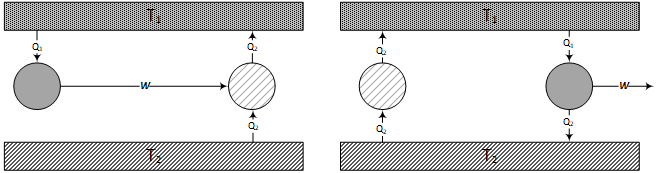
\includegraphics[width=\textwidth]{img/enunciados-2ley.png}
	\caption{Máquinas térmicas imposibles; izquierda (a), derecha (b). $T_2<T_1$.}
	\label{fig:maquinas-imposibles}
\end{figure}

\par De la desigualdad de Clausius podemos derivar una forma diferencial de la segunda ley.
\par Consideremos primero un ciclo compuesto por una rama reversible $1\xrightarrow{R}2$ y otra irreversible $2\xrightarrow{I}1$. Luego otro ciclo, pero completamente reversible $1\xrightarrow{R}2\xrightarrow{R}1$ (Fig.\ \ref{fig:ciclos-entropia}), que por el.

\begin{figure}[htb!]
	\centering
	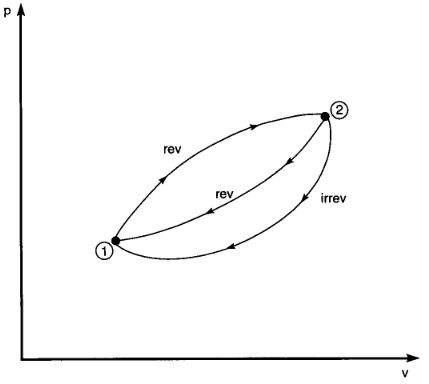
\includegraphics[width=0.45\textwidth]{img/entropia.png}
	\label{fig:ciclos-entropia}
	\caption{Dos ciclos: uno reversible y otro semi-reversible.}
\end{figure}

\par Para el primer ciclo tenemos, según la desigualdad de Clausius
\begin{equation*}
	\displaystyle\int_{1}^{2}\left(\frac{\delta Q}{T}\right)_R+\displaystyle\int_{2}^{1}\left(\frac{\delta Q}{T}\right)_I\leq0.
\end{equation*}
\par Para el segundo,
\begin{gather*}
	\displaystyle\int_{1}^{2}\left(\frac{\delta Q}{T}\right)_R+\displaystyle\int_{2}^{1}\left(\frac{\delta Q}{T}\right)_R=0\\
	\displaystyle\int_{1}^{2}\left(\frac{\delta Q}{T}\right)_R=-\displaystyle\int_{2}^{1}\left(\frac{\delta Q}{T}\right)_R,
\end{gather*}
reemplazando en la desigualdad del primer ciclo, tenemos
\begin{gather*}
	-\displaystyle\int_{2}^{1}\left(\frac{\delta Q}{T}\right)_R+\displaystyle\int_{2}^{1}\left(\frac{\delta Q}{T}\right)_I\leq0\\
	\displaystyle\int_{2}^{1}\left(\frac{\delta Q}{T}\right)_R\geq\displaystyle\int_{2}^{1}\left(\frac{\delta Q}{T}\right)_I.
\end{gather*}
Como la desigualdad vale entre dos estados arbitrarios, también aplica para los integrandos, entonces
\begin{equation*}
	\left(\frac{\delta Q}{T}\right)_R\geq\left(\frac{\delta Q}{T}\right)_I,
\end{equation*}
que por (\ref{eq:dS})
\begin{equation}\label{eq:dif-segunda-ley}
	dS\geq\frac{\delta Q}{T}.
\end{equation}
Donde la igualdad vale para procesos reversibles.
\vspace{2mm}
\par Este resultado nos permite identificar si un sistema es o no es capaz de evolucionar a través de cierto proceso. Un proceso es posible si satisface (\ref{eq:dif-segunda-ley}); si lo hace a través de la igualdad es reversible e irreversible si satisface la desigualdad. Por otro lado, si encontramos un proceso que satisfaga la desigualdad en sentido contrario, entonces afirmamos que es un proceso \emph{imposible}.

\par Para un sistema completamente aislado $\delta Q=0$, entonces
\begin{equation*}
	dS\geq0\qquad S_f\geq S_i.
\end{equation*}

\par Los sistemas siempre evolucionan a un estado de mayor entropía, se dice que un sistema aislado está en equilibrio cuando alcanza un estado de máxima entropía.
\par Notar que si el sistema aislado está compuesto por otros subsistemas, en ellos es posible encontrar procesos que disminuyan su entropía; pero lo hacen a expensas de los otros subsistemas que aumentaran su entropía al menos hasta igualar el déficit del primero.

\section{Formas especiales de escribir la segunda ley}

\begin{itemize}
	\item Transformaciones isotérmicas finitas. ($\Delta U=0$)
	      \begin{gather*}
		      \Delta S\geq\frac{1}{T}\int_{i}^{f}\delta Q\\
		      \Rightarrow \Delta S\geq\frac{Q}{T},\qquad\Delta S\geq\frac{-W}{T}.
	      \end{gather*}
	\item Transformaciones adiabáticas. ($\delta Q=0$)
	      \begin{equation*}
		      dS\geq0.
	      \end{equation*}
	\item Transformaciones isoentrópicas. ($dS=0$)
	      \begin{equation*}
		      \delta Q\leq0.
	      \end{equation*}
	      Notar que un proceso adiabático reversible es isoentrópico.
	\item Transformaciones isocóricas.
	      \par De la primera ley, $dV=0\implies\delta Q=c_{V}dT$,
	      \begin{equation*}
		      dS\geq c_{V}\frac{dT}{T},\qquad\Delta S\geq c_{V}\ln{\frac{T_f}{T_i}}
	      \end{equation*}
	\item Transformaciones isobáricas.
	      \par En este caso, $delta Q=c_{p}dT$ y,
	      \begin{equation*}
		      dS\geq c_{p}\frac{dT}{T},\qquad \Delta S\geq c_{p}\ln{\frac{T_f}{T_i}}
	      \end{equation*}
\end{itemize}

\section{Relaciones fundamentales: funciones de Gibbs y Hemholtz}
Considerando la siguiente forma de escribir la primera ley
\begin{equation*}
	\delta Q=C_{p}dT-Vdp.
\end{equation*}
Combinando con (\ref{eq:dif-segunda-ley}),
\begin{equation*}
	TdS\geq C_{p}dT-Vdp.
\end{equation*}
Recordando que $C_{p}=dH/dT$,
\begin{equation*}
	TdS\geq dH-Vdp,
\end{equation*}
o
\begin{equation}\label{eq:def-dG}
	dH\leq TdS+Vdp
\end{equation}
\par Similarmente, de $delta Q=C_{V}dT+pdV$, arribamos a
\begin{equation*}
	TdS\geq dU+\delta W,
\end{equation*}
o
\begin{equation}\label{eq:def-dF}
	dU\leq TdS-pdV
\end{equation}
\par Esto nos induce a introducir dos nuevas funciones: la de Hemholtz, $F=U-TS$; y la de Gibbs, $G=H-TS=U+pV-TS$. Debido a que tanto $S=S(T,V)$ como $U=U(T)$, son funciones de estado, $F=F(T,V)$ y $G=G(T,V)$ también lo son. La ventaja de estas funciones es poder expresar a las ecuaciones (\ref{eq:def-dG}) y (\ref{eq:def-dF}) en términos de $T$ y $V$ como variables independientes. Utilizando las funciones de Hemholtz y de Gibbs, respectivamente, redefinimos:
\begin{gather}
	dF\leq-SdT-pdV \label{eq:dF}\\
	dG\leq-SdT+Vdp \label{eq:dG}
\end{gather}

\subsubsection{Interpretación de las funciones}
Si consideramos procesos \emph{isotérmicos},
\begin{equation*}
	dF\leq\delta W;
\end{equation*}
es decir que $F$ es la energía disponible para realizar trabajo.
\par Si consideramos ahora procesos \emph{isotérmicos} e \emph{isobáricos} simultáneamente (por ejemplo, cambios de fase)
\begin{equation*}
	dG=0,
\end{equation*}
por lo cual $G$ {\sl se conserva}.
\par Decimos que las relaciones (\ref{eq:def-dG})-(\ref{eq:dG}) son las {\sc relaciones fundamentales}.

\subsection{Condiciones de equilibrio termodinámico}
En un sistema que se encuentre en un estado de \emph{equilibrio estable} no es posible la ocurrencia de procesos naturales (o espontáneos); o son reversibles, o son imposibles. En cambio, si se encuentra en un \emph{equilibrio inestable}, se abre la posibilidad a los procesos irreversibles.\\
Podemos vincular estas definiciones con la segunda ley de la termodinámica y definir una serie de condiciones que caracterizan el equilibrio termodinámico.
\begin{gather*}
	dU\leq TdS-pdV\\
	dH\leq TdS+Vdp\\
	dF\leq -SdT-pdV\\
	dG\leq -SdT+Vdp\\
	dS\geq\frac{\delta Q}{T}
\end{gather*}
Donde la igualdad vale para procesos reversibles y la desigualdad para los irreversibles.
\par Esto significa que cuando un sistema tiende al equilibrio, $G,\, F,\, H$ y $U$ tienden a un mínimo y $S$ a un máximo.
\par Si el sistema evolucionara hacia un mínimo de $S$ y un máximo del resto, entonces se tratase de un proceso imposible.

\subsection{Relación entre entropía y temperatura potencial}
Recordando que
\begin{equation*}
	\theta=T \left(\frac{1000}{p}\right)^{R/c_{p}}
\end{equation*}
Diferenciando de manera logarítmica
\begin{equation}\label{eq:cp.dlnteta}
	c_{p}d\ln{\theta}=c_{p}d\ln{T}-Rd\ln{p}
\end{equation}
\par Por otro lado, de la primera ley tenemos
\begin{equation*}
	\frac{\delta Q}{T}=Cp\frac{dT}{T}-mR\frac{dp}{p}
\end{equation*}
o para procesos reversibles,
\begin{equation}\label{eq:ds.Tp}
	ds=c_{p}\frac{dT}{T}-R\frac{dp}{p}
\end{equation}
donde $s$ es la \emph{entropía específica}.
\par Igualando (\ref{eq:cp.dlnteta}) y (\ref{eq:ds.Tp})
\begin{equation}
	ds=c_{p}d\ln{\theta},\qquad s=c_{p}\ln{\theta}+\mathrm{constante}
\end{equation}
\par Podemos decir entonces, que los procesos adiabáticos reversibles son isoentrópicos. Para procesos adiabáticos \emph{irreversibles} $ds>0$ y $d\theta=0$; en este caso, el incremento de entropía viene dado por el trabajo irreversible (por ejemplo, la disipación de energía cinética por fricción).

\begin{equation*}
	\mathsf{PROCESO\, ISOENTROPICO}\implies\mathsf{PROCESO\, ADIABATICO}
\end{equation*}

\chapter{El Agua y sus Transformaciones}
\section{Sistemas Heterogéneos}
Para un sistema homogéneo, dos propiedades intensivas pueden describir sus estado termodinámico. Por lo tanto, solo dos variables de estado pueden variar independientemente; entonces un sistema homogéneo tiene dos grados de libertad termodinámicos. Para un sistema heterogéneo, cada fase se puede pensar como un subsistema homogéneo abierto, de modo que permita el intercambio con las otras fases del sistema. Luego, el número de propiedades intensivas que describen el estado termodinámico del sistema heterogéneo es proporcional al número de fases presentes.
\par Si consideramos una mezcla de aire seco y vapor de agua, la cual se encuentra en estado gaseoso y también se encuentra condensada; tenemos un sistema heterogéneo de dos componentes: aire seco y agua.
\par Este sistema heterogéneo puede ser descripto convenientemente en términos de propiedades extensivas que dependen de la cantidad de cada componente presente. Una propiedad extensiva $Z$ del sistema se puede escribir como la contribución de cada fase:
\begin{equation}\label{eq:Zs}
	Z_{s}=Z_{g}+Z_{c},
\end{equation}
donde los subíndices $g$ y $c$ hacen alusión a los subsistemas gaseoso y condensado que incluyen tanto al aire seco como al vapor de agua. La propiedad extensiva del subsistema gaseoso se puede especificar por su presión, temperatura y la cantidad de moles de aire seco y vapor de agua
\begin{equation*}
	Z_{g}=Z_{g}(p,T,n_{d},n_{v}).
\end{equation*}
Si la fase condensada es agua pura, la podemos determinar por su presión, temperatura y la cantidad de moles de agua condensada
\begin{equation*}
	Z_{c}=Z_{c}(p,T,n_{c}).
\end{equation*}
Luego los cambios de la propiedad $Z$ de cada subsistema son
\begin{gather}
	dZ_{g}=\frac{\partial Z_{g}}{\partial T}dT+\frac{\partial Z_{g}}{\partial p}dp+\frac{\partial Z_{g}}{\partial n_{d}}dn_{d}+\frac{\partial Z_{g}}{\partial n_{v}}dn_{v}\label{eq:dZg}\\
	dZ_{c}=\frac{\partial Z_{c}}{\partial T}dT+\frac{\partial Z_{c}}{\partial p}dp+\frac{\partial Z_{c}}{\partial n_{c}}dn_{c}\label{eq:dZc},
\end{gather}
donde $dn_{d}$, $dn_{v}$ y $dn_{c}$ representan el cambio en la cantidad de moles de cada elemento.
\par Es conveniente introducir una variable de estado que mida como cambia $Z$ en todo el sistema con el incremento de uno de sus componentes, es decir en procesos isobáricos e isotérmicos. Definimos así a la \emph{propiedad parcial molar} o \emph{potencial químico} como la tasa a la cual cambia una propiedad extensiva con respecto al cambio de la cantidad de moles de las $k$ componentes bajo condiciones isobáricas e isotérmicas.
\begin{equation}\label{eq:Zk}
	\overline{Z}_{k}=\left(\frac{\partial Z}{\partial n_{k}}\right)_{pTn},
\end{equation}
donde el subíndice $k$ se refiere a una determinada fase y componente.
\par Para sistemas cerrados, la cantidad de moles de cada componente permanece constante,
\begin{gather}
	dn_{d}=0\label{eq:dnd-0},\\
	d(n_{v}+n_{c})=0\label{eq:dnvnc-0}.
\end{gather}
Sumando (\ref{eq:dZg}) y (\ref{eq:dZc}) y agregando los resultados recién vistos, tenemos el cambio total de la propiedad $Z$ sobre el sistema:
\begin{equation}\label{eq:dZtot}
	dZ_{tot}=\frac{\partial Z_{tot}}{\partial T}dT+\frac{\partial Z_{tot}}{\partial p}dp+(\overline{Z}_{v}-\overline{Z}_{c})dn_{v}.
\end{equation}

\section{Equilibrio Químico}
Utilizando las herramientas que describimos arriba, definimos ahora un criterio para estudiar el equilibrio químico de un sistema heterogéneo. El \emph{potencial químico} para las $k$ especies $\mu_{k}$ está definido como función de Gibbs parcial molar.
\begin{equation}\label{eq:pot-quimk}
	\mu_{k}=\overline{G}_{k}=\frac{\partial G}{\partial n_{k}}.
\end{equation}
De (\ref{eq:dZg}) tenemos
\begin{equation}\label{eq:dGg}
	dG_{g}=\frac{\partial G_{g}}{\partial T}dT+\frac{\partial G_{g}}{\partial p}dp+\mu_{d}dn_{d}+\mu_{v}dn_{v}.
\end{equation}
Si tenemos en cuenta las relaciones fundamentales,
\begin{equation}\label{eq:dGg-SV}
	dG_{g}=-S_{g}dT+V_{g}dp+\mu_{d}dn_{d}+\mu_{v}dn_{v}.
\end{equation}
Observar que las expresiones anteriores solo involucran variables de estado, por lo tanto solo dependen si hubo o no hubo cambios de fase. La ecuación anterior describe el cambio de la función de Gibbs para la fase gaseosa.
\par Similarmente, para la parte condensada llegamos a
\begin{equation}\label{eq:dGc-SV}
	dG_{c}=-S_{c}dT+V_{c}dp+\mu_{c}dn_{c}.
\end{equation}
\par Sumando ambas fases tenemos el cambio total de la función de Gibbs, si consideramos además procesos reversibles o irreversibles, podemos extender la relación fundamental de Gibbs a
\begin{equation}\label{eq:dG-relfundamental}
	dG_{tot}\leq-S_{tot}dT+V_{tot}dp+(\mu_{v}-\mu_{c})dn_{v},
\end{equation}
donde aplica la igualdad para procesos reversibles y la desigualdad para irreversibles. Para que el sistema se encuentre en equilibrio, la función de Gibbs debe minimizarse. Consideremos un cambio de fase a presión y temperatura constante, durante el cambio tendremos una variación de $dn_{v}$ que puede ser positiva si hay evaporación, negativa si hay condensación. Según los criterios de equilibrio que definimos, los procesos posibles conducen a la función de Gibbs a un mínimo.
\begin{equation*}
	dG\leq(\mu_{v}-\mu_{c})dn_{v},
\end{equation*}
entonces, debe valer:
\begin{itemize}
	\item Si hay evaporación, $dn_{v}\geq0,\quad\mu_{v}\leq\mu_{c}.$
	\item Si hay condensación, $dn_{v}\leq0,\quad\mu_{v}\geq\mu_{c}$.
\end{itemize}
Cuando el sistema alcanza el equilibrio, la función de Gibbs alcanza un mínimo $(dG=0)$, entonces
\begin{equation}\label{eq:mu-equim}
	\mu_{v}=\mu_{c},
\end{equation}
lo cual llamamos \emph{equilibrio químico} e implica que los potenciales químicos sean iguales. Si hay diferencia entre ellos, existirá un flujo de masa de la fase de mayor $\mu$ a la fase menor $mu$, hasta equilibrar los potenciales.

\section{Relaciones fundamentales para sistemas de muchas componentes}
De igual manera que utilizamos la función de Gibbs anteriormente, todas las relaciones fundamentales definidas para sistemas homogéneos pueden ser generalizadas para sistemas heterogéneos de $C$ componentes y $P$ fases.

\begin{gather*}
	dU=TdS-pdV+\sum_{j=1}^{P}\sum_{i=1}^{C}\mu_{ij}dn_{ij},\\
	dH=TdS+Vdp+\sum_{j=1}^{P}\sum_{i=1}^{C}\mu_{ij}dn_{ij},\\
	dF=-SdT-pdV+\sum_{j=1}^{P}\sum_{i=1}^{C}\mu_{ij}dn_{ij},\\
	dG=-SdT+Vdp+\sum_{j=1}^{P}\sum_{i=1}^{C}\mu_{ij}dn_{ij},
\end{gather*}
donde introducimos las expresiones alternativas para el potencial químico de la componente $i$ y la fase $j$
\begin{equation*}
	\mu_{ij}=\left(\frac{\partial U}{\partial n_{ij}}\right)_{SVn}=\left(\frac{\partial H}{\partial n_{ij}}\right)_{Spn}=\left(\frac{\partial F}{\partial n_{ij}}\right)_{TVn}=\left(\frac{\partial G}{\partial n_{ij}}\right)_{pTn}.
\end{equation*}
Notar que solo la última de ellas corresponde a un proceso isobárico e isotérmico. Por ende, las restantes no representan propiedades parciales molares de acuerdo a la definición (\ref{eq:Zk}). Teniendo en cuenta que los cambios de fase a presión constante también ocurren bajo temperatura constante, la última de las expresiones para potencial químico es la conveniente, y por tanto la ecuación (\ref{eq:dG-CP}) es la mejor para describir cambios de fase.
\par Para un sistema cerrado, la masa de cada componente se conserva, entonces
\begin{equation*}
	\sum_{j=1}^{P}dn_{ij}=0,\qquad i=1,\cdots,C.
\end{equation*}
Luego, para una componente $i$, teniendo en cuenta que $dn_{i1}=-\sum_{j=2}^{P}dn_{ij}$
\begin{align*}
	\sum_{j=1}^{P}\mu_{ij}dn_{ij} & =\mu_{i1}dn_{i1}+\sum_{j=2}^{P}\mu_{ij}dn_{ij} \\
	                              & =\sum_{j=2}^{P}(\mu_{ij}-\mu{i1})dn_{ij},
\end{align*}
donde $j=1$ representa una fase arbitraria para esa componente $i$. Entonces el conjunto de relaciones fundamentales las podemos escribir tal que

\end{document}
